\chapter{The Lungs and Gas Exchange}\label{ch:g7:lungs-and-gas-exchange}

Every minute of your life, about eight litres of air pass
through two organs you have never seen. \Cref{ch:g4:breathing}
sketched the path and the swap; \cref{ch:g7:how-animals-breathe}
placed the human machine among the kingdom's four. This
chapter completes the picture: the ventilation machinery,
the air pockets by their proper name, the numbers of the
exchange --- and what smoke does to the whole works.

\section{The ventilation machinery}

\begin{proposition}[How air is moved]\label{prop:g7:lungs-and-gas-exchange:ventilation}
The \omterm{def:g7:how-animals-breathe:four}{lungs} have no \omterm{def:g3:bones-and-muscles:muscle}{muscles} of their own; the chest pumps
them like a bellows:
\begin{itemize}
  \item \omterm{def:g7:what-is-respiration:respiration}{breathing} in is \emph{work}: the \omterm{def:g3:bones-and-muscles:skeleton}{rib} \omterm{def:g3:bones-and-muscles:muscle}{muscles} lift
        and widen the cage, and the
        \emph{diaphragm}\index{diaphragm} --- the broad
        \omterm{def:g3:bones-and-muscles:muscle}{muscle} floor under the \omterm{def:g7:how-animals-breathe:four}{lungs} --- flattens
        downward; the widened chest stretches the \omterm{def:g7:how-animals-breathe:four}{lungs},
        and air flows in to fill them;
  \item \omterm{def:g7:what-is-respiration:respiration}{breathing} out, at rest, is mostly \emph{release}:
        \omterm{def:g3:bones-and-muscles:muscle}{muscles} relax, the stretched chest springs back,
        air flows out. (Blowing out candles adds \omterm{def:g3:bones-and-muscles:muscle}{muscle}
        to the spring.)
\end{itemize}
About $15$ times a minute at rest
(\cref{def:g4:breathing:movements}), unasked
(\cref{rem:g5:brain-in-command:more}) --- and deepened
and quickened on demand
(\cref{prop:g7:organs-at-work:supply}).
\end{proposition}
\admitted

\begin{example}[Feeling the bellows]\label{ex:g7:lungs-and-gas-exchange:feel}
Hands on \omterm{def:g3:bones-and-muscles:skeleton}{ribs}, breathe in deep: the cage rises and widens
under your palms (\cref{ex:g4:breathing:watch}). Now pant
like a dog: the quick shallow puffs are almost all
\omterm{prop:g7:lungs-and-gas-exchange:ventilation}{diaphragm}. Hiccups, for completeness, are the \omterm{prop:g7:lungs-and-gas-exchange:ventilation}{diaphragm}'s
twitchy false starts --- the bellows misfiring on its own
schedule.
\end{example}

\section{The alveoli and the exchange}

\begin{definition}[Alveoli]\label{def:g7:lungs-and-gas-exchange:alveoli}
The tiny air pockets of \cref{def:g4:breathing:organs} are
the \emph{alveoli}\index{alveolus}: hundreds of millions
of thin-walled bubbles clustered at the airways' finest
tips, each wrapped in fine \omterm{def:g4:heart-and-blood:vessels}{blood vessels}. Their summed
surface is the half tennis court of
\cref{rem:g4:breathing:sponge} --- the human copy of
\cref{prop:g7:how-animals-breathe:spec}'s
large-thin-moist specification.
\end{definition}

\begin{proposition}[The exchange, in numbers]\label{prop:g7:lungs-and-gas-exchange:numbers}
Compare the air that enters with the air that \omterm{def:g1:plants-around-us:parts}{leaves}:
inhaled air is about $21$ percent \omterm{def:g7:what-is-respiration:respiration}{oxygen} and almost free
of \omterm{def:g7:what-is-respiration:respiration}{carbon dioxide}; exhaled air is down to about $16$
percent \omterm{def:g7:what-is-respiration:respiration}{oxygen} and up to about $4$ percent \omterm{def:g7:what-is-respiration:respiration}{carbon
dioxide} (warm and moist besides ---
\cref{ex:g4:breathing:mirror}). The differences are the
exchange: across the alveolar walls, \omterm{def:g7:what-is-respiration:respiration}{oxygen} crosses to
the \omterm{prop:g4:journey-of-food:absorb}{blood} and \omterm{def:g7:what-is-respiration:respiration}{carbon dioxide} crosses back
(\cref{prop:g4:breathing:exchange}), every minute of
every day.
\end{proposition}
\admitted

\begin{omfigure}
\begin{tikzpicture}
  \node[anchor=south west, inner sep=0] (img) at (0,0)
    {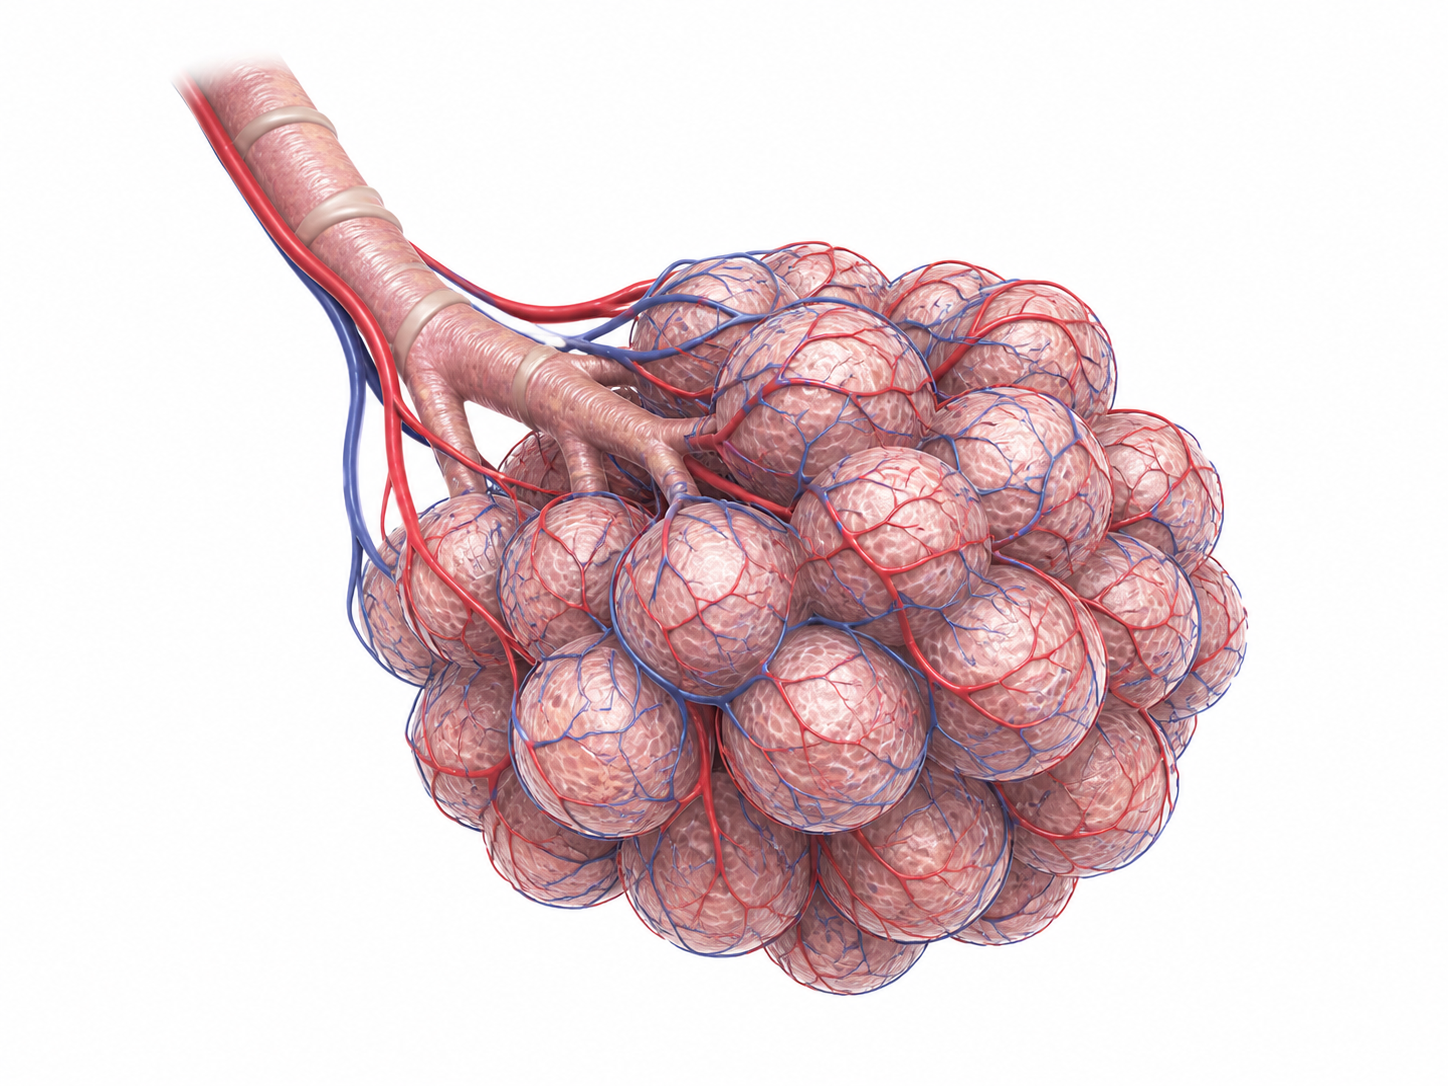
\includegraphics[width=0.6\linewidth]{images/book1/ai/fig-alveoli.png}};
  \begin{scope}[x={(img.south east)}, y={(img.north west)},
      every node/.style={font=\small}]
    \draw[omDef, thick] (0.24,0.83) -- (0.12,0.94)
      node[above] {finest airway};
    \draw[omThm, thick] (0.78,0.62) -- (0.90,0.80)
      node[above, align=center, omThm] {the wrapping\\ fine vessels};
    \draw[omMeth!60!black, thick] (0.46,0.34) -- (0.30,0.01)
      node[below, align=center, omMeth!60!black]
      {across each bubble's thin wall:\\ oxygen to the blood, carbon\\
       dioxide back to the air};
  \end{scope}
\end{tikzpicture}

{\small One alveolar cluster of the hundreds of millions: thin
bubble walls, a wrap of fine \omterm{def:g4:heart-and-blood:vessels}{vessels}, and the two-way crossing
that is the point of it all.}
\end{omfigure}

\begin{example}[The accounting checks]\label{ex:g7:lungs-and-gas-exchange:accounting}
Eight litres a minute, a twentieth of each breath's \omterm{def:g7:what-is-respiration:respiration}{oxygen}
kept: the arithmetic supplies roughly the resting body's
\omterm{def:g7:what-is-respiration:respiration}{oxygen} bill --- and in effort, with \omterm{def:g7:what-is-respiration:respiration}{breathing} tripled and
deepened and the \omterm{def:g4:heart-and-blood:heart}{heart}'s rounds accelerated
(\cref{prop:g7:organs-at-work:supply}), the delivery
multiplies to match the \omterm{def:g3:bones-and-muscles:muscle}{muscles}' bill. The machine's
numbers and the body's ledger balance; they are the same
books kept at two counters.
\end{example}

\section{The machinery abused: smoke}

\begin{proposition}[What smoke does to the works]\label{prop:g7:lungs-and-gas-exchange:smoke}
Tobacco smoke attacks every floor of this chapter
(\cref{prop:g5:healthy-choices:substances} gave the
warning; here is the engineering):
\begin{itemize}
  \item its tars coat and irritate the airways: the
        cleaning surfaces falter and the ``smoker's
        cough'' is the airways' overloaded broom;
  \item alveolar walls, chronically irritated, break
        down: pockets merge into fewer, bigger, baggier
        spaces --- \emph{surface is lost}, and with it
        exchange (the specification, dismantled);
  \item one of smoke's gases rides the \omterm{prop:g4:journey-of-food:absorb}{blood}'s \omterm{def:g7:what-is-respiration:respiration}{oxygen}
        seats, crowding \omterm{def:g7:what-is-respiration:respiration}{oxygen} off its own transport;
  \item and the airways narrow --- every breath through a
        smoker's chest is a breath through a part-blocked
        bellows.
\end{itemize}
The damage is slow, cumulative and only partly
reversible: the never-started \omterm{def:g7:how-animals-breathe:four}{lung} keeps its half tennis
court whole (\cref{rem:g5:healthy-choices:never}).
\end{proposition}
\admitted

\begin{example}[Two stair tests]\label{ex:g7:lungs-and-gas-exchange:stairs}
The three flights of \cref{ch:g7:organs-at-work}, taken
by two adults of equal age and training habits, one a
long-term smoker: the smoker arrives gasping at a \omterm{prop:g4:heart-and-blood:pulse}{pulse}
the other reaches only sprinting. Less surface, seats
taken, narrowed airways --- the supply chain pays
\cref{prop:g7:organs-at-work:bill}'s bill through a
throttled intake. Fitness tests read the \omterm{def:g7:how-animals-breathe:four}{lungs}' history
as surely as any scan.
\end{example}

\begin{method}[Keeping the machinery]\label{met:g7:lungs-and-gas-exchange:keep}
\Cref{met:g4:breathing:care}, upgraded with this
chapter's reasons:
\begin{enumerate}
  \item no smoke --- yours or others': surface lost is
        barely regained;
  \item air the rooms (\cref{exo:g4:breathing:10}) and
        prefer clean outdoor air for sport;
  \item exercise the bellows: \omterm{def:g7:what-is-respiration:respiration}{deep-breathing} effort
        builds the \omterm{def:g7:what-is-respiration:respiration}{breathing} \omterm{def:g3:bones-and-muscles:muscle}{muscles} and keeps the full
        surface ventilated;
  \item \omterm{def:g7:what-is-respiration:respiration}{nose-breathing} in cold and dust
        (\cref{exo:g4:breathing:7}) --- the filter
        protects the broom.
\end{enumerate}
\end{method}

\section{Exercises}

\begin{exercise}[$\star$]\label{exo:g7:lungs-and-gas-exchange:1}
Describe \omterm{def:g7:what-is-respiration:respiration}{breathing} in and \omterm{def:g7:what-is-respiration:respiration}{breathing} out as work and
release: which \omterm{def:g3:bones-and-muscles:muscle}{muscles}, which movements?
\end{exercise}

\begin{exercise}[$\star$]\label{exo:g7:lungs-and-gas-exchange:2}
What is the \omterm{prop:g7:lungs-and-gas-exchange:ventilation}{diaphragm}, and where does it sit?
\end{exercise}

\begin{exercise}[$\star$]\label{exo:g7:lungs-and-gas-exchange:3}
What are the \omterm{def:g7:lungs-and-gas-exchange:alveoli}{alveoli} --- how many, how walled, wrapped
in what?
\end{exercise}

\begin{exercise}[$\star$]\label{exo:g7:lungs-and-gas-exchange:4}
Give the round numbers: \omterm{def:g7:what-is-respiration:respiration}{oxygen} in inhaled air, in
exhaled air; \omterm{def:g7:what-is-respiration:respiration}{carbon dioxide} in exhaled air. What are the
differences?
\end{exercise}

\begin{exercise}[$\star$]\label{exo:g7:lungs-and-gas-exchange:5}
Which specification do the \omterm{def:g7:lungs-and-gas-exchange:alveoli}{alveoli} meet, and with which
two other organs of this year do they share it?
\end{exercise}

\begin{exercise}[$\star$]\label{exo:g7:lungs-and-gas-exchange:6}
Name three of smoke's four attacks on the machinery.
\end{exercise}

\begin{exercise}[$\star\star$]\label{exo:g7:lungs-and-gas-exchange:7}
Why is \omterm{def:g7:what-is-respiration:respiration}{breathing} in work while resting \omterm{def:g7:what-is-respiration:respiration}{breathing} out is
free? Where does the outward push come from?
\end{exercise}

\begin{exercise}[$\star\star$]\label{exo:g7:lungs-and-gas-exchange:8}
Explain why lost alveolar surface cannot be compensated
by \omterm{def:g7:what-is-respiration:respiration}{breathing} faster --- which factor of the exchange is
missing?
\end{exercise}

\begin{exercise}[$\star\star$]\label{exo:g7:lungs-and-gas-exchange:9}
Interpret the two stair tests of
\cref{ex:g7:lungs-and-gas-exchange:stairs} attack by
attack.
\end{exercise}

\begin{exercise}[$\star\star$]\label{exo:g7:lungs-and-gas-exchange:10}
A diver breathes out slowly while surfacing; a trumpet
player holds long steady notes. Which halves of
\cref{prop:g7:lungs-and-gas-exchange:ventilation} are
they each training or using?
\end{exercise}

\begin{exercise}[$\star\star$]\label{exo:g7:lungs-and-gas-exchange:11}
Reconcile \cref{ex:g7:lungs-and-gas-exchange:accounting}
with \cref{prop:g7:organs-at-work:supply}: which three
adjustments multiply delivery in effort, and at which
counters?
\end{exercise}

\begin{exercise}[$\star\star\star$]\label{exo:g7:lungs-and-gas-exchange:12}
``The \omterm{def:g7:how-animals-breathe:four}{lung} is a border of half a tennis court folded
into a shoebox, and smoke is a slow fire at the
border.'' Justify both images with this chapter's
numbers and mechanisms.
\end{exercise}

\section{Problem: The Breathing Machine Dossier}

\begin{problem}[{Weekend problem --- an engineer's
inspection of the human bellows}]\label{pb:g7:lungs-and-gas-exchange:1}
An engineering class ``inspects'' the human \omterm{def:g7:what-is-respiration:respiration}{breathing}
machine on paper: intake, pump, exchange surface,
transport connection, and maintenance record.

\medskip\noindent\textbf{Part I --- The pump.}
\begin{enumerate}
  \item Draw up the pump's cycle: the two phases, the
        movers of each, and which phase costs \omterm{prop:g3:balanced-diet:jobs}{energy} at
        rest.
  \item The pump has no contact with the pumped organ's
        own \omterm{def:g3:bones-and-muscles:muscle}{muscle} --- the \omterm{def:g7:how-animals-breathe:four}{lungs} have none. How does the
        chest's widening move air at all?
  \item Give the pump's resting rate and its two effort
        adjustments
        (\cref{prop:g7:organs-at-work:supply}).
  \item Panting, sighing, blowing out candles: assign
        each to its place in the cycle's mechanics.
\end{enumerate}

\medskip\noindent\textbf{Part II --- The exchange
surface.}
\begin{enumerate}[resume]
  \item Specify the surface: name, number, wall,
        wrapping, summed size.
  \item Verify the specification against
        \cref{prop:g7:how-animals-breathe:spec}, item by
        item.
  \item The intake air and exhaust air differ by the
        chapter's percentages. Compute the \omterm{def:g7:what-is-respiration:respiration}{oxygen}
        difference as a fraction of the intake's $21$
        percent --- roughly what share of inhaled \omterm{def:g7:what-is-respiration:respiration}{oxygen}
        is kept?
  \item Why must the exhaust stay warm and moist ---
        which property of the surface is that the price
        of?
\end{enumerate}

\medskip\noindent\textbf{Part III --- The maintenance
record.}
\begin{enumerate}[resume]
  \item File smoke's four attacks under: intake, pump,
        surface, transport. One line each.
  \item The dossier notes: ``surface losses are
        capital losses.'' Explain, against the coughs
        and colds that are running repairs.
  \item Write the maintenance schedule ---
        \cref{met:g7:lungs-and-gas-exchange:keep} --- as
        four engineer's directives with reasons.
  \item Conclude the inspection: one sentence on why
        this machine, alone of the body's pumps and
        borders, is half under the owner's voluntary
        control --- and what that control is for
        (speech, song, the diver's slow exhale).
\end{enumerate}
\end{problem}
